%\documentclass[12pt]{article}
%\usepackage[a4paper, margin=1in]{geometry} 
%\usepackage{graphicx} 
%\usepackage{hyperref}
%\usepackage{float}
%\usepackage{multicol}
%\usepackage{multirow}
%\usepackage{amsmath}
%\usepackage[font=small, labelfont=bf]{caption}
%
%\begin{document}

%
% PAM – accepted mutations
%
\subsection{PAM – accepted mutations}
PAM is a popular scoring scheme for protein sequence alignments. It is based on substitution matrices created from experiment data.

%
% Accepted point mutations
%
\subsubsection*{Accepted point mutations}
\begin{itemize}
\item Independent of positions and neighbor residues
\item Independent from previous mutations at the same position
\item Biological clock is assumed (the rate of mutations is constant)
\end{itemize}

%
% PAM (point accepted mutation) 
%
\subsubsection*{PAM (point accepted mutation)}
One PAM means one accepted point mutation per 100 residues. 

\noindent
Resources of constructing a PAM score
\begin{itemize}
\item 34 super-families
\item 71 groups of homologous sequences (85\% identity) 
\end{itemize}

%
% Preparations for constructing a PAM score
%
\subsubsection*{Preparations for constructing a PAM score}
Counting the number of mutations is the fist step to make a PAM score. Several sub-steps are involved.

\begin{itemize}
\item Create a phylogenetic tree
\item Estimate ancestor sequences
\item Count all occurrences of mutations
\end{itemize}

%
% Frequencies of estimated mutations
%
\subsubsection*{Frequencies of estimated mutations}
Frequencies of estimated mutations are counted in internal nodes of the reconstructed tree. \\

$\begin{aligned}
f_{ab} &: \text{The number of mutations from } a \text{ to } b \text{ or from } b \text{ to } a \\
f_{a} &: \text{The total number of mutations in which a takes part} \\
f & : \text{Twice the total number of mutations}
\end{aligned} $

%
% Example of frequency calculation
%
\subsubsection*{Example of frequency calculation}
Calculate $f_{CA}$, $f_{C}$, and $f$ from the phylogenetic tree and the table below.

\begin{figure}[H]
  \centering
      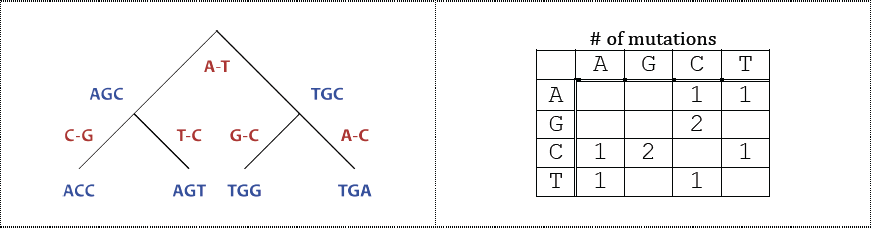
\includegraphics[width=0.75 \textwidth]{fig11/scoring_mat_frequency_example.png}
  \caption{Phylogenetic tree and a table of the number of mutations}
\end{figure}

$\begin{aligned}
f_{CA} &=1 \\
f_{C} &= 1 + 2 + 1 = 4\\
f &= 10
\end{aligned} $

%
% Background frequencies
%
\subsubsection*{Background frequencies}
The background probabilities are calculated from the data source. 

$\begin{aligned}
p_a &: \text{The relative occurrence of a in the observed sequences} 
\end{aligned} $

%
% Example of background frequencies
%
\subsubsection*{Example of background frequencies}
Calculate $p_G$ from the sequences below.

\begin{verbatim}
   Seq1 ACC
   Seq2 AGT
   Seq3 TGG
   Seq4 TGA
\end{verbatim}

$p_G = \dfrac{4}{12} \approx 0.333$

\bigskip 

%\end{document}
